\documentclass[tikz]{standalone}
\usetikzlibrary{positioning, arrows.meta}
\usepackage{wasysym}
\begin{document}
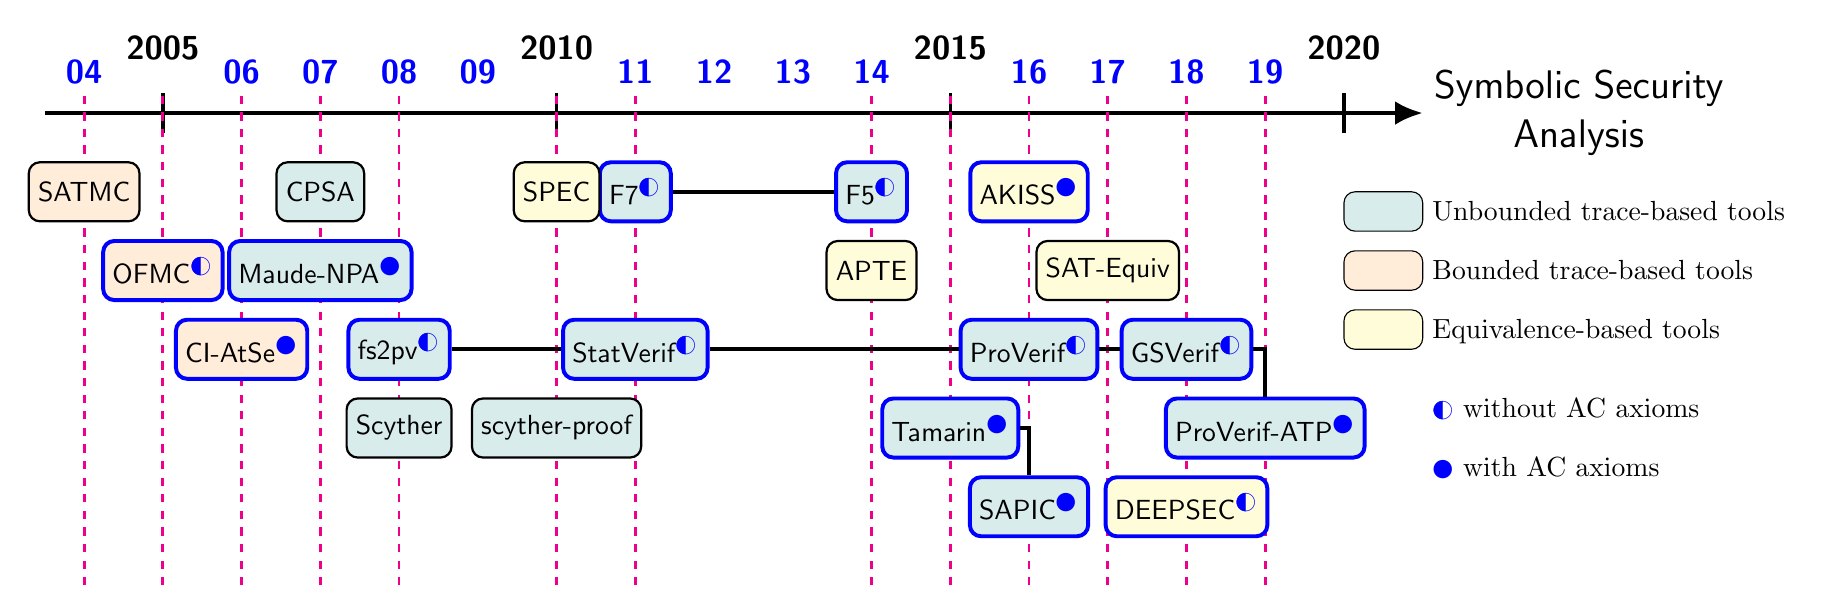
\begin{tikzpicture}[
	% Define a node distance for consistent spacing
	node distance=1cm and 2cm,
	% Style for the event description boxes
	event/.style={
		rectangle,
		rounded corners=4pt,
		draw=black,
		thick,
		fill=blue!20,
		text width=6cm,
		align=center,
		font=\sffamily,
		minimum height=1cm
	},
	event2/.style={
		rectangle,
		rounded corners=4pt,
		draw=black,
		thick,
		fill=orange!20,
		text width=8cm,
		align=center,
		font=\sffamily,
		minimum height=1cm
	},
	event3/.style={
		rectangle,
		rounded corners=4pt,
		draw=black,
		thick,
		fill=teal!20,
		text width=8cm,
		align=center,
		font=\sffamily,
		minimum height=1cm
	},
	% Style for the year markers on the axis
	year/.style={
		font=\sffamily\bfseries\large,
		anchor=south
	},
	node/.style={
		rectangle,
		rounded corners=4pt,
		draw=black,
		thick,
		fill=white,
%		text width=8cm,
		align=center,
		font=\sffamily,
		minimum height=.75cm
	},
	unbounded/.style={
		rectangle,
		rounded corners=4pt,
		draw=black,
		thick,
		fill=teal!15,
		align=center,
		font=\sffamily,
		minimum height=.75cm
	},
	bounded/.style={
		rectangle,
		rounded corners=4pt,
		draw=black,
		thick,
		fill=orange!15,
		align=center,
		font=\sffamily,
		minimum height=.75cm
	},
	equiv/.style={
		rectangle,
		rounded corners=4pt,
		draw=black,
		thick,
		fill=yellow!15,
		align=center,
		font=\sffamily,
		minimum height=.75cm
	}
	]
	% Draw the main horizontal timeline axis with a nice arrow tip
	\draw[line width=1.5pt, -{Latex[length=3.5mm, width=3mm]}] (-1.5,0) -- (16,0) node[right, font=\Large\sffamily, align=center] {Symbolic Security\\ Analysis};
	
	\draw[fill=teal!15, rounded corners=4pt] (15,-1.5) rectangle (16,-1) node[below right] {Unbounded trace-based tools};
	\draw[fill=orange!15, rounded corners=4pt] (15,-2.25) rectangle (16,-1.75) node[below right] {Bounded trace-based tools};
	\draw[fill=yellow!15, rounded corners=4pt] (15,-3) rectangle (16,-2.5) node[below right] {Equivalence-based tools};
	\draw[draw=white, rounded corners=4pt] (15,-4) rectangle (16,-3.5) node[below right] {$\color{blue}{\LEFTcircle}$ without AC axioms};
	\draw[draw=white, rounded corners=4pt] (15,-4.75) rectangle (16,-4.25) node[below right] {$\color{blue}{\CIRCLE}$ with AC axioms};
%	\node at (17,-3.5) {$\color{blue}^{\LEFTcircle}$ without AC axioms};
%	\node at (17,-4.25) {$\color{blue}^{\CIRCLE}$ with AC axioms};
	
	
	% Use a loop to place the years and tick marks on the axis
	\foreach \x/\yeartext in {0/2005, 5/2010, 10/2015, 15/2020}{
		\draw[line width=1.2pt] (\x, -0.25) -- (\x, 0.25);
		\node[year, above=0.3cm of {\x,0.25}] {\yeartext};
	}
	
	% Position the event nodes relative to coordinates on the timeline
%	\draw[red, fill=red] (8,0) circle (2.5pt) node[below=.25cm] {NOW};
	\node[year, above=0cm of {-1,0.25}, blue] {04};
	\node[year, above=0cm of {1,0.25}, blue] {06};
	\node[year, above=0cm of {2,0.25}, blue] {07};
	\node[year, above=0cm of {3,0.25}, blue] {08};
	\node[year, above=0cm of {4,0.25}, blue] {09};
	\node[year, above=0cm of {6,0.25}, blue] {11};
	\node[year, above=0cm of {7,0.25}, blue] {12};
	\node[year, above=0cm of {8,0.25}, blue] {13};
	\node[year, above=0cm of {9,0.25}, blue] {14};
	\node[year, above=0cm of {11,0.25}, blue] {16};
	\node[year, above=0cm of {12,0.25}, blue] {17};
	\node[year, above=0cm of {13,0.25}, blue] {18};
	\node[year, above=0cm of {14,0.25}, blue] {19};
	
	\foreach \x in {-1,0, ..., 3,5,6,9,10,...,14}{
		\draw[line width=1pt, dashed, magenta] (\x, -6) -- (\x, 0.25);
	}
%	\draw[line width=1.5pt, dashed, blue] (-1, -6) -- (-1, 0.25);
%	\draw[line width=1.5pt, dashed, blue] (0, -6) -- (0, 0.25);
	
	\node[unbounded] at (2,-1) {CPSA}; % 07
	\node[unbounded, draw=blue, line width=.5mm] (F7) at (6,-1) {F7$\color{blue}^{\LEFTcircle}$}; % 11
	\node[unbounded, draw=blue, line width=.5mm] (F5) at (9,-1) {F5$\color{blue}^{\LEFTcircle}$}; % 14
	\node[unbounded, draw=blue, line width=.5mm] at (2,-2) {Maude-NPA$\color{blue}^{\CIRCLE}$}; % 07
	\node[unbounded, draw=blue, line width=.5mm] (ProVerif) at (11,-3) {ProVerif$\color{blue}^{\LEFTcircle}$}; % 16
	\node[unbounded, draw=blue, line width=.5mm] (fs2pv) at (3,-3) {fs2pv$\color{blue}^{\LEFTcircle}$}; % 08
	\node[unbounded, draw=blue, line width=.5mm] (GSVerif) at (13,-3) {GSVerif$\color{blue}^{\LEFTcircle}$}; % 18
	\node[unbounded, draw=blue, line width=.5mm] (ProVerif-ATP) at (14,-4) {ProVerif-ATP$\color{blue}^{\CIRCLE}$}; % 19
	\node[unbounded, draw=blue, line width=.5mm] (StatVerif) at (6,-3) {StatVerif$\color{blue}^{\LEFTcircle}$}; % 11
	\node[unbounded] at (3,-4) {Scyther}; % 08
	\node[unbounded] at (5,-4) {scyther-proof}; % 10
	\node[unbounded, draw=blue, line width=.5mm] (Tamarin) at (10,-4) {Tamarin$\color{blue}^{\CIRCLE}$}; % 13
	\node[unbounded, draw=blue, line width=.5mm] (SAPIC) at (11,-5) {SAPIC$\color{blue}^{\CIRCLE}$}; % 14
	\node[bounded, draw=blue, line width=.5mm] at (1,-3) {CI-AtSe$\color{blue}^{\CIRCLE}$}; % 06
	\node[bounded, draw=blue, line width=.5mm] at (0,-2) {OFMC$\color{blue}^{\LEFTcircle}$}; % 05
	\node[bounded] at (-1,-1) {SATMC}; % 04
	\node[equiv, draw=blue, line width=.5mm] at (11,-1) {AKISS$\color{blue}^{\CIRCLE}$}; % 16
	\node[equiv] at (9,-2) {APTE}; % 14
	\node[equiv, draw=blue, line width=.5mm] at (13,-5) {DEEPSEC$\color{blue}^{\LEFTcircle}$}; % 18
	\node[equiv] at (12,-2) {SAT-Equiv}; % 17
	\node[equiv] at (5,-1) {SPEC}; % 10
	
	\draw[line width=1.5pt] (F7.east) to (F5.west);
	\draw[line width=1.5pt] (Tamarin.east) -| (SAPIC.north);
	\draw[line width=1.5pt] (fs2pv.east) -| (StatVerif.west);
	\draw[line width=1.5pt] (StatVerif.east) -| (ProVerif.west);
	\draw[line width=1.5pt] (ProVerif.east) -| (GSVerif.west);
	\draw[line width=1.5pt] (GSVerif.east) -| (ProVerif-ATP.north);
	
%	\node[
%		rectangle,
%		rounded corners=4pt,
%		draw=black,
%		thick,
%		fill=blue!20,
%		text width=4cm,
%		align=center,
%		font=\sffamily,
%		minimum height=1cm, 
%		below=of {3,-1.5}, align=center
%	] (event2) {\textbf{SHA-3 hash function}};
%	
%	\draw[->, thick, gray] (event2.north) -- (3,0);
%	\node[event, below=of {1,0}, align=center] (event1) {\textbf{Scalar multiplication for Curve25519}};


%	\node[event, below=of {7,-4.5}, align=center] (event4) {\bfseries Mutivariate Quadratic based Signatures: Mayo2};

%	\node[event2, below=of {6,-1}, align=center] (event5) {\bfseries Schnorr protocol in Jasmin\\ \normalfont (José Bacelar Almeida, Denis Firsov, Tiago Oliveira, and Dominique Unruh)};
	
%	\draw[->, thick, orange, dashed] (event5.north) -- (6,0);
%	\node[event3, below=of {8,-4}, align=center] (event6) {\bfseries Forking Lemma in EasyCrypt\\ \normalfont (Denis Firsov, Jakub Janků)};
%	\draw[->, thick, teal, dashed] (event6.south) -- (8,-8);
	
\end{tikzpicture}
\end{document}